\subsection{T-reX tool}\label{sec:results-T-reX}

An example of the output from the application of T-reX has been included in the supplementary material in~\autoref{sec:supplementary}. The manipulated \texttt{ecoinvent} databases, which are the main product of T-reX, can be recreated by following the instructions in the package documentation~\citep{mcdowall2023T-reXdocs}.

\subsection{Case study: Li-ion batteries}\label{sec:results-casestudy}

As described in~\autoref{sec:method-casestudy}, this case study calculated the waste and material footprints (with a variety of other indicators) for the unaltered background inventories of five Li-ion batteries with the functional unit being 1~kg of the battery at the global market. The purpose of this simple case study was to test, verify, and demonstrate the functionality and limitations of T-reX. This section includes some highlights of the results, with full results included in the supplementary material (\autoref{sec:supplementary}). Because the `pseudo-LCIA' methods created by T-reX are integrated into the user's \texttt{brightway} project as if they were standard LCIA methods, the footprint calculations can be performed in the customary way. In the supplementary material, there are screenshots of selected results obtained using the \texttt{ActivityBrowser} software, including contribution analysis and a Sankey diagram that disaggregates the final footprint result over the activities in the supply chain.

\subsubsection{Sankey visualisation of flows in waste and material inventory footprints}\label{sec:results-case_study-sankey}

\autoref{fig:sankey_waste} presents a Sankey diagram depicting the supply chain flows of `total solid waste' attributed to the NMC 811 Li-ion battery at the global market in the \texttt{ecoinvent} database version 3.9.1. As the supply chains are expansive, this visualisation has been greatly simplified for print, the full version is included in the supplementary material~\autoref{sec:supplementary}. As is evident in the figure, the largest contributors to the waste footprint are the extraction and processing of the raw materials, with the largest flows coming from the extraction of cobalt, lithium, and nickel. Due to the nature of LCA, the waste flows do not represent the `real' physical flows directly, but rather an abstraction thereof based on, in this case, economic allocation---the market price of the functional unit produced by the activity~\citep{guinee2004economicallocation}. If an unallocated database were available, the waste flows could be calculated with T-reX in the same way and be more directly related to the physical flows of the activities.

\begin{figure}[H]
    \centering
    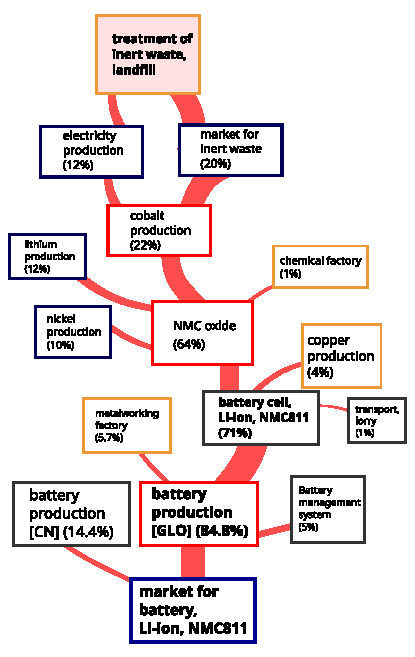
\includegraphics[width=8cm]{figures/T-reX_NMC811_WasteTotalSolid.pdf}
    \caption{A simplified Sankey diagram showing the total solid waste footprint flows for the NMC 811 battery supply chain at the global market in the \texttt{ecoinvent} database version 3.9.1.}\label{fig:sankey_waste}
\end{figure}

\subsubsection{Temporal and scenario variation in waste and material inventory footprints}
%\label{sec:results-case_study-total_footprints}

%! total
\autoref{fig:waste_totalANDcarbon} (a) shows the `total solid waste' inventory footprint for the five Li-ion batteries in the case study from 2020 to 2100 under the SSP2 scenario using the baseline and PkBudg500 RCPs of the REMIND model. The NMC811 battery has the largest footprint, producing over 50~kg of waste per kilogram of battery produced. The  LiMn\(_2\)O\(_4\) battery has the smallest footprint, producing less than 4~kg of waste per kilogram of battery. In each case, there was only a slight downward trend in the waste footprints between 2020 and 2100. This is mostly in the period between 2020 and 2040 and could be attributable to the relatively rapid decrease in fossil-fuel use that is factored into the models over this time (since many produce relatively large amounts of waste during extraction and combustion). For the total waste generated by these batteries, there was very little difference observed between the baseline and PkBudg500 RCPs.

%! CO2
The inclusion of carbon capture and storage (CCS) in the prospective databases is apparent in~\autoref{fig:waste_totalANDcarbon} (b), with the rapid increase in the production of carbon dioxide `waste' over the period from 2020--2040 that is not seen in the baseline scenario. This result highlights the fact that the (often) downward trends in global warming impacts calculated with prospective databases using standard LCIA methods are dependent on the assumptions made about the introduction of CCS technology. The actual deployment of these technologies was only around 37~Mt CO$_2$/yr as of 2023~\citep{dziejarski2023ccs}, far short of the levels projected in many of the RCP scenarios~\citep{sacchi2023premisedocs}. The authors consider that the over representation of CCS and the under representation of waste processing technologies in the prospective databases is one significant limitation to the validity of prospective LCA databases.
%!!!!

\begin{figure}[H]
    \centering
    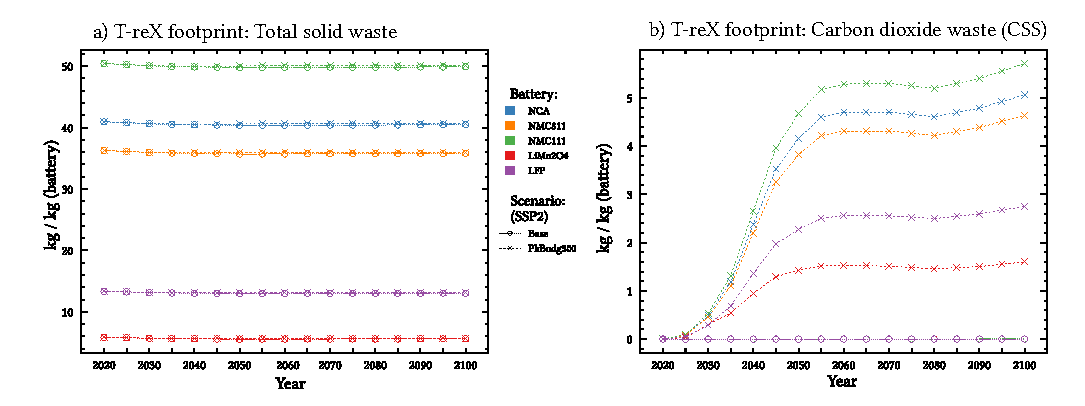
\includegraphics[width=16cm]{figures/T-reX-wastefootprint-totalANDcarbon.pdf}
    \caption{T-reX calculated supply chain inventories for the five Li-ion batteries in the case study, showing their `footprints' for: (a) total solid waste, and (b) carbon dioxide waste (from carbon capture and storage (CCS) only). The footprints were modelled with prospective LCA databases from 2020 to 2100 under the SSP2 scenario using the baseline and PkBudg500 RCPs of the REMIND model.}\label{fig:waste_totalANDcarbon}
\end{figure}
%!!!!

\subsubsection{Contribution of `top-processes' in the supply chain}%\label{sec:results-case_study-topprocesses}

\autoref{fig:top_contribution} shows the contribution of the `top-processes' to the graphite footprint of the  LiMn\(_2\)O\(_4\) battery under the baseline scenario from 2020--2100. The total footprint is seen to more than triple, from 0.16~kg/kg in 2020 to 0.52~kg/kg in 2050 and onward to 2100. The largest contributor is not, in this case, the battery-embedded graphite electrode (which is the second top process), but `silicon production' from further up in the supply chain. This result is likely a reflection of the electrification of the transport and energy sectors that is included in the REMIND model. The results of this kind of analysis with T-reX can be used to identify the most significant processes in the supply chain and to target interventions to reduce the potential environmental impact of production.

\begin{figure}[H]
    \centering
    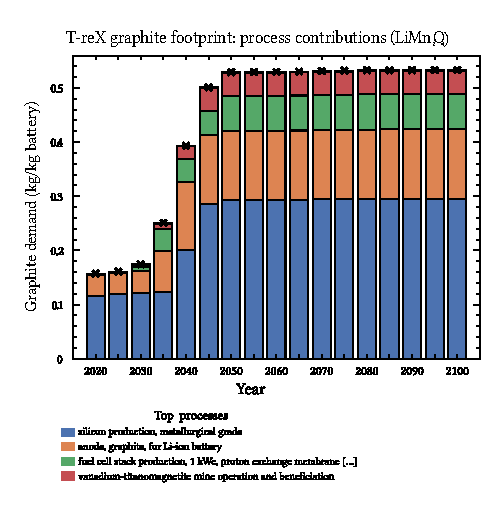
\includegraphics[width=9cm]{figures/T-reX-wastefootprint-processcontributions.pdf}
    \caption{Contribution by the `top-processes' to graphite demand inventory of the LiMn\(_2\)O\(_4\) battery from 2020 to 2100 under the SSP2 scenario using the baseline RCPs of the REMIND model.}\label{fig:top_contribution}
\end{figure}

%!!!!

\subsubsection{Contribution of industrial sectors in the supply chain}\label{sec:results-case_study-topsectors}

\autoref{fig:cpc_contribution} shows the contribution of sectors (grouped by CPC codes) to the total natural gas footprint of the LFP battery under the PkBudg500 pathway. In this example, the relative contribution of the sector `47160: Electronic integrated circuits' is seen to decrease from 11\% in 2020 to 8\% in 2100, while over the same period the contribution of the sector `46430: Parts of primary cells, primary batteries and electrodes' increases from 32\% to 38\%. The method used to calculate these contributions involves traversing the supply chain branches to a certain level (max. 4, in this case), cutting a specified point (5\% in this case), and grouping the value of the `leaves' by their CPC code. The results, therefore, will depend on how deeply the user would like to inspect the supply chain. Additionally, the utility of these results is dependent on how well the CPC codes define the processes in the supply chain for the particular case.

\begin{figure}[H]
    \centering
    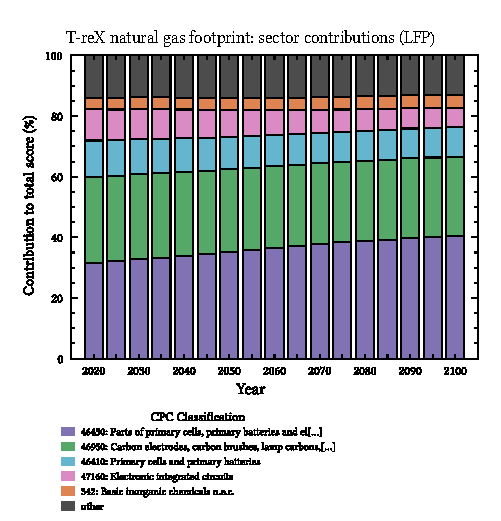
\includegraphics[width=9cm]{figures/T-reX-wastefootprint-sectorcontributions.pdf}
    \caption{Contribution of industrial sectors to the natural gas footprint of the LFP battery from 2020 to 2100 under the SSP2 scenario using the baseline RCP of the REMIND model.}\label{fig:cpc_contribution}
\end{figure}


\subsubsection{Comparison with `similar' LCIA methods}\label{sec:results-case_study-methodcomparison}

A comparison of the results from T-reX's `Coal (black)' demand method with the LCIA method `EDIP 2003 - coal no LT' is shown in~\autoref{fig:comparison_methods}. In this case, both the trends and the magnitude of the scores were very similar, both demonstrating a general decrease in the use of coking coal in the battery's footprints. Such comparability was also observed for other fossil-fuel-related methods (e.g., natural gas and petroleum), and to a lesser extent, for some of the metal demand methods (e.g., zinc and cobalt). Correlation between standard LCIA methods and T-reX methods is not generally to be expected, however, due to fundamental differences in the way that the methods are constructed. In standard LCIA methods, impact scores are derived exclusively from the magnitude of the exchanges between the biosphere and the technosphere, that is, extraction and emission. In the T-reX methods, the footprint scores are based on an accounting of either waste generated or material demand, both of which are technosphere-technosphere exchanges in terms of LCA modelling. For the material demand methods especially, this distinction is critical. For example, the application of the EDIP 2003 or the CSP methods for a given metal will provide a score that is proportional to the amount extracted by mining, whereas the T-reX method provides an aggregation of the exchanges with the market for that metal. The T-reX method, therefore, considers cases of co-production, recycling, and substitution, providing a picture of the supply chain pressures that are not captured by the standard LCIA methods. This makes the T-reX methods more sensitive to the modeling choices (e.g.,economic allocation) that are generally embedded in LCA databases.

\begin{figure}[H]
    \centering
    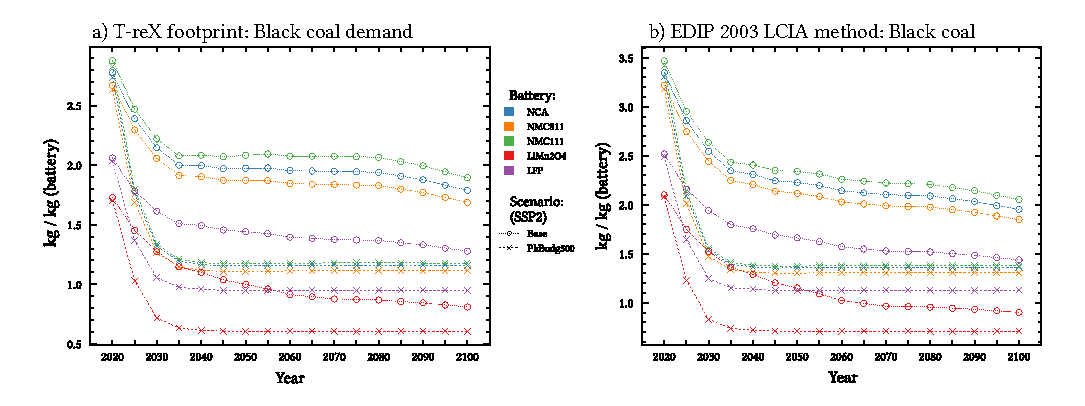
\includegraphics[width=16cm]{figures/T-reX-coalANDedip.pdf}
    \caption{Comparison of the (a) `T-reX - Coal (black)' demand footprint with the (b) conventional LCIA method `EDIP 2003 - coal no LT'  in the case study from 2020 to 2100 under the SSP2 scenario using the baseline and PkBudg500 RCPs of the REMIND model for all five batteries.}\label{fig:comparison_methods}
\end{figure}

\subsubsection{Comparison with other studies}\label{sec:results-case_study-comparison}

In the most similar published method, \cite{laurenti2023wastefootprint} used an alternative procedure for calculating the waste footprint of \~1400 activities in the \texttt{ecoinvent} database version 3.5. Direct comparison is not possible, as this database contains only one generic Li-ion battery, `market for battery, Li-ion, rechargeable, prismatic'. The inventory of this battery most closely resembles that of the NMC 111 battery in this case study. \autoref{tab:results-case_study-comparison} presents a comparison of the results from the two studies, where possible. For liquid, solid, and recycled waste, the results were closely aligned, however, for the hazardous waste fraction, Laurenti et al. reported 95\%, whereas T-reX reported only 3\%. The reason for this discrepancy is explained by the fact that in the method of Laurenti et al.\, a ``waste flow was regarded as hazardous when the hazardousness was clearly stated in its subsequent waste treatment activity''. The authors continue: ``It should be noted that the high hazardousness ratios for many products might indicate a weakness in the validity of this measure''. In T-reX, the source database is deconstructed into a list of separate exchanges, and only those explicitly defined as hazardous are marked as such.

\begin{table}[H]
    \centering
    \caption{Comparison of the results from the T-reX battery case study (database: \texttt{ecoinvent} 3.9.1 REMIND SSP2 Base 2020, activity: Li-ion NMC 111) with those from \cite{laurenti2023wastefootprint} (database: \texttt{ecoinvent} 3.5, activity:`Li-ion').}\label{tab:results-case_study-comparison}
    \begin{tabular}{lll}
        \toprule
        \textbf{Indicator}         & \textbf{T-reX} & \textbf{Laurenti et al.} \\
        \midrule
        Total solid waste (kg/kg)  & 50.9           & 62.5                     \\
        Total liquid waste (kg/kg) & 3.53           & 3.63                     \\
        Hazardous waste (kg/kg)    & 1.47           & 62.6                     \\
        Recycled waste (kg/kg)     & 1.59           & 1.98                     \\
        \bottomrule
    \end{tabular}
\end{table}

